\documentclass[submit]{harvardml}

% FDV: Make sure all front matter has correct years, dates, book sections, etc.
\course{CS181-S22}
\assignment{Assignment \#2}
\duedate{7:59pm EST, Feb 25th, 2022}

\usepackage[OT1]{fontenc}
\usepackage[colorlinks,citecolor=blue,urlcolor=blue]{hyperref}
\usepackage[pdftex]{graphicx}
%\usepackage{subfig}
\usepackage{fullpage}
\usepackage{amsmath}
\usepackage{amssymb}
\usepackage{framed}
\usepackage{color}
\usepackage{soul}
\usepackage{todonotes}
\usepackage{listings}
\usepackage{common}
\usepackage{enumitem}
\usepackage{bm}
\newcommand{\B}{\text{B}}
\newcommand{\Beta}{\text{Beta}}

\usepackage[mmddyyyy,hhmmss]{datetime}

\usepackage{subcaption}
\newcommand{\TODO}{{\color{red}TODO }}

\definecolor{verbgray}{gray}{0.9}

\lstnewenvironment{csv}{%
  \lstset{backgroundcolor=\color{verbgray},
  frame=single,
  framerule=0pt,
  basicstyle=\ttfamily,
  columns=fullflexible}}{}

\begin{document}

\begin{center}
{\Large Homework 2: Classification and Bias-Variance Trade-offs}\\
\end{center}

\subsection*{Introduction}

This homework is about classification and bias-variance trade-offs. In
lecture we have primarily focused on binary classifiers trained to
discriminate between two classes. In multiclass classification, we
discriminate between three or more classes.  Most of the material for Problem 1 and Problem 3, and all of the material for Problem 2 will be covered by the end of the Tuesday 2/8 lecture. The rest of the material will be covered by the end of the Thursday 2/10 lecture.  We encourage you to read
CS181 Textbook's Chapter 3 for more information on linear
classification, gradient descent, classification in the discriminative
setting (covers multiclass logistic regression and softmax), and
classification in the generative setting. Read Chapter 2.8 for more
information on the trade-offs between bias and variance.

As a general note, for classification problems we imagine that we have
the input matrix $\boldX \in \reals^{N \times D}$ (or perhaps they
have been mapped to some basis $\bm{\Phi}$, without loss of
generality) with outputs now ``one-hot encoded."  This means that if
there are~$K$ output classes, rather than representing the output
label $y$ as an integer~${1,2,\ldots,K}$, we represent $\boldy$ as a
``one-hot" vector of length~$K$. A ``one-hot" vector is defined as
having every component equal to 0 except for a single component which
has value equal to 1.  For example, if there are $K = 7$ classes and a
particular data point belongs to class 3, then the target vector for
this data point would be~$\boldy = [0,0,1,0,0,0,0]$.  We will define
$C_1$ to be the one-hot vector for the 1st class, $C_2$ for the 2nd
class, etc.  Thus, in the previous example $\boldy = C_3$. If there
are $K$ total classes, then the set of possible labels is $\{C_1
\ldots C_K \} = \{C_k\}_{k=1}^K$.  Throughout the assignment we will
assume that each label $\boldy \in \{C_k\}_{k=1}^K$ unless otherwise
specified. The most common exception is the case of binary classification
($K = 2$), in which case labels are the typical integers $y \in \{0, 1\}$.\\

In problems 1 and 3, you may use \texttt{numpy} or \texttt{scipy}, but
not \texttt{scipy.optimize} or \texttt{sklearn}. Example code given is
in Python 3.\\

Please type your solutions after the corresponding problems using this
\LaTeX\ template, and start each problem on a new page.\\

Please submit the \textbf{writeup PDF to the Gradescope assignment `HW2'}. Remember to assign pages for each question.  \textbf{You must include your plots in your writeup PDF. } The supplemental files will only be checked in special cases, e.g. honor code issues, etc. \\

Please submit your \textbf{\LaTeX\ file and code files to the Gradescope assignment `HW2 - Supplemental'}. 

%%%%%%%%%%%%%%%%%%%%%%%%%%%%%%%%%%%%%%%%%%%%%
% Problem 1
%%%%%%%%%%%%%%%%%%%%%%%%%%%%%%%%%%%%%%%%%%%%%

\begin{problem}[Exploring Bias and Variance, 10 pts]
  In this problem, we will explore the bias and variance of a
  few different model classes when it comes to logistic regression.

  Consider the true data generating process $y \sim \text{Bern}(f(x)), f(x) = 0.4 \times \sin(1.2x) + 0.5$, where $x \in [-3, 3]$, and $y \in \{0,1\}$.
  Recall that for a given $x$, bias and variance are defined in terms of expectations \textit{over randomly drawn datasets} $D$
  from this underlying data distribution:
  \begin{align*}
  \text{Bias}[\hat{f}(x)] &= \mathbb{E}_D[\hat{f}(x)] - f(x)\\
  \text{Variance}[\hat{f}(x)] &= \mathbb{E}_D[(\hat{f}(x) - \mathbb{E}_D[\hat{f}(x)])^2]
  \end{align*}
  Here, $\hat{f}(x)$ is our estimator (learned through logistic
  regression on a given dataset $D$).  We will directly explore the
  bias-variance trade-off by drawing multiple such datasets and
  fitting different logistic regression models to each.  Remember that
  we, the modelers, do not usually see the true data distribution.
  Knowledge of the true $f(x)$ is only exposed in this problem to (1)
  make possible the simulation of drawing multiple datasets, and (2)
  to serve as a pedagogical tool in allowing verification of the true
  bias.

\begin{enumerate}

\item Consider the three bases $\phi_1(x) = [1, x]$, $\phi_2(x) = [1,
  x, x^2]$, $\phi_3(x) = [1, x, x^2, x^3, x^4, x^5]$.  For each
  of these bases, generate 10 datasets of size $N = 30$ using the
  starter code provided, and fit a logistic regression model using
  sigmoid($w^T \phi(x)$) to each dataset by using gradient descent to
  minimize the negative log likelihood.  This means you will be
  running gradient descent 10 times for each basis, once for each
  dataset.  Note that the classes are represented with 0's and 1's.
  
  Use random starting values of $w$, $\eta=0.001$, take 10,000 update
  steps for each gradient descent run, and make sure to average the
  gradient over the data points (for each step). These parameters,
  while not perfect, will ensure your code runs in a reasonable amount
  of time. The emphasis of this problem is on capturing the
  bias-variance trade-off, so don't worry about attaining perfect
  precision in the gradient descent as long as this trade-off is
  captured in the final models.

   Note: Overflow RuntimeWarnings due to \verb|np.exp| should be safe to ignore, if any. Also, to reduce stress from randomness in students' solutions (due to randomized weight initialization differences), in line $109$ of the \verb|T2_P1.py| starter code, we call \verb|np.random.seed(1738)| to set a deterministic random seed. Please do not change this! In addition, please do not change the randomized weight initialization code in lines $42-46$.

\item Create three plots, one for each basis. Starter code is available which you may modify.
By default, each plot displays three types of functions:
(1) the true data-generating distribution $f(x)$ (the probability that $y=1$ for different $x$).
(2) all 10 of the prediction functions learned from each randomly drawn dataset, and
(3) the mean of the 10 prediction functions.
Moreover, each plot also displays 1 of the randomly generated datasets and highlights the corresponding prediction function learned by this dataset.

\item How are bias and variance reflected in the 3 types of curves on
  the graphs?  How do the fits of the individual and mean prediction
  functions change?  Keeping in mind that none of the model classes
  match the true generating process exactly, discuss the extent to
  which each of the bases approximates the true process.

  Note: In this problem, we are not interested in whether the model is
  more biased for certain inputs $x$ compared to other inputs $x'$.
  We are interested in the overall bias and variance of $\hat{f}(x)$
  across the different basis choices. In other words, we want to investigate how the bias between $\hat{f}(x)$ and the ground truth as well as the variance of $\hat{f}(x)$ will be different over different basis choices. 

\item If we were to increase the size of each dataset drawn from $N = 30$ to a larger number, how would the variance change? The bias?   Why might this be the case?

\end{enumerate}

\end{problem}

\newpage

\subsection*{Solution}

\begin{enumerate}
	\item See supplemental code.
	
	\item See Figure \ref{fig:problem 1}.
	
		\begin{figure}[h]
			\centering
			\begin{subfigure}[b]{0.475\textwidth}
				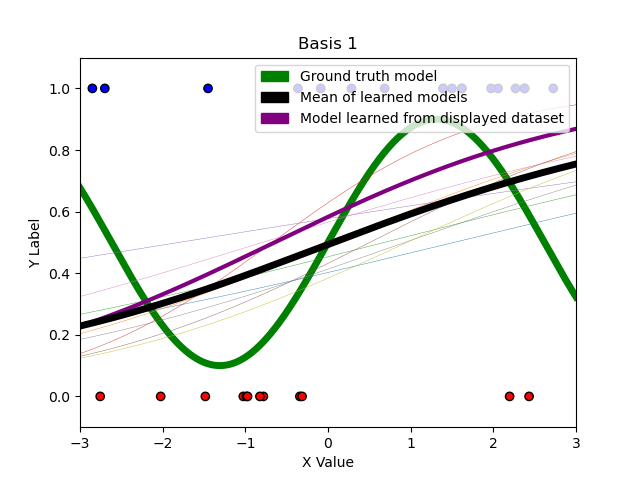
\includegraphics[width=\textwidth]{Basis 1}
			\end{subfigure}
			\hfill
			\begin{subfigure}[b]{0.475\textwidth}
				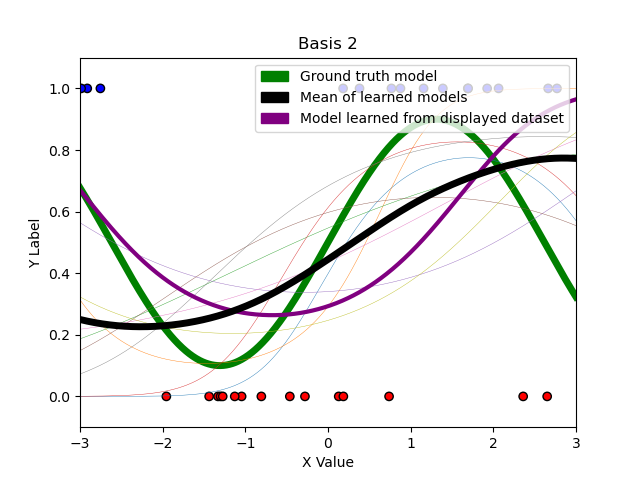
\includegraphics[width=\textwidth]{Basis 2}
			\end{subfigure}
			\hfill
			\vskip\baselineskip
			\begin{subfigure}[b]{0.475\textwidth}
				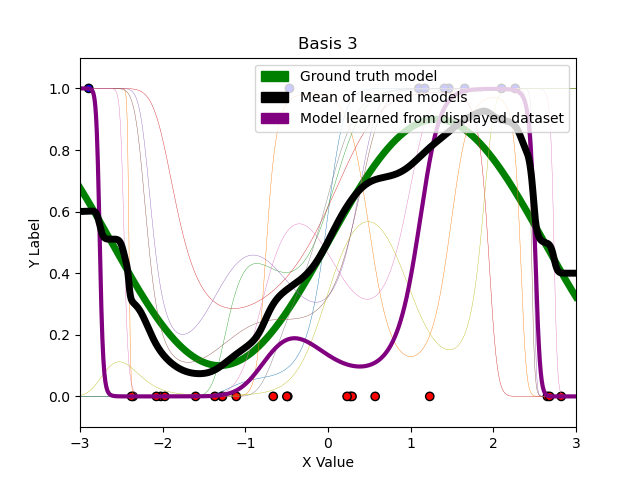
\includegraphics[width=\textwidth]{Basis 3}
			\end{subfigure}
			\caption{Logistic regressions for various bases}
			\label{fig:problem 1}
		\end{figure}
	
	\item In each graph, the bias of the model class is indicated by the difference between the mean of learned models and the ground truth model, while the variance is indicated by the variability between the ten models in each class, including the model learned from the displayed dataset. From this, we can see that the model class with basis $\phi_1$ has a very high bias, since the mean is dissimilar to the ground truth model, and a very low variance, since all of the ten models look similar. The model class with basis $\phi_2$ has moderate bias and variance, since its mean is somewhat close to the ground truth and the models are roughly similar but have variability. The model class with basis $\phi_3$ has a very low bias, since its mean fits the ground truth model almost exactly, but a very high variance, since its individual models vary wildly. In general, we can see that increasing the size of the model decreases variance while increasing bias. Basis $\phi_1$ does a poor job of approximating the true process since it underfits the data both on average and for individual models. Basis $\phi_2$ does a mediocre job both on average and in individual models. Basis $\phi_3$ does a very good job on average, but dramatically overfits the data in individual models, meaning any given individual model is not a good approximation of the true process. Overall, if only one individual model had to be chosen to approximate the true process, one given by $\phi_2$ would be best, but not ideal, and if an average over multiple models could be chosen, the average of those given by $\phi_3$ would be ideal.
	
	\item Increasing the size of each data set would decrease the variance for all of the model classes, especially the model class with highest variance. The overall decrease comes from the fact that as more data points are provided, the data are more likely to be similar across data sets, since they better represent the ground truth, and so the individual models in each class would be more similar to each other. Perhaps more importantly, the variance would decrease most in higher-variance model classes, especially the model class using $\phi_3$, because as more data points are introduced, its models have less ``room" to overfit the data, and must instead become close to the ground truth model, so they will tend to be more similar.
	
	By contrast, increasing the size of each dataset would not significantly improve the bias for any of the model classes. This is because the means of the model classes for bases $\phi_1$ and $\phi_2$ are essentially already as close to the ground truth as they can be, given the parameters available to them. In particular, the ground truth model looks as though it can be closely approximated by at least third-degree polynomial, but the first two basis have at most first- and second-order polynomials, respectively. The bias of the model class using $\phi_3$ would improve as its models better approximate the ground truth model, but the mean of the model class is already so close to the ground truth that this increase would not be too significant.

\end{enumerate}

%%%%%%%%%%%%%%%%%%%%%%%%%%%%%%%%%%%%%%%%%%%%%
% Problem 2
%%%%%%%%%%%%%%%%%%%%%%%%%%%%%%%%%%%%%%%%%%%%%

\begin{problem}[Maximum likelihood in classification, 15pts]

  Consider now a generative $K$-class model.  We adopt class prior
  $p(\boldy = C_k; \bpi) = \pi_k$ for all $k \in \{1, \ldots, K\}$
(where $\pi_k$ is a parameter of the prior).
Let  $p(\boldx|\boldy=C_k)$ denote
the class-conditional density of features $\boldx$ (in this
case for class $C_k$). Consider the data set $D = \{(\boldx_i,
\boldy_i)\}_{i=1}^n$ where as above $\boldy_i \in \{C_k\}_{k=1}^K$ is
encoded as a one-hot target vector and the data are independent.

\begin{enumerate}
  \item Write out the log-likelihood of the data set, $\ln p(D ; \bpi)$.

  \item Since the prior forms a distribution, it has the constraint that
    $\sum_k\pi_k - 1 = 0$.  Using the hint on
Lagrange multipliers below, give the
    expression for the maximum-likelihood estimator for the prior
    class-membership probabilities, i.e.
    $\hat \pi_k.$
    Make sure to write out the intermediary equation you need
    to solve to obtain this estimator. Briefly state why your final answer is intuitive.
\end{enumerate}

    For the remaining questions, let the
    class-conditional probabilities be Gaussian distributions with
the same covariance matrix
    $$p(\boldx | \boldy = C_k) = \mathcal{N}(\boldx |  \bmu_k, \bSigma), \text{\ for\ }k \in \{1,\ldots, K\}$$
    and different means $\bmu_k$ for each class.

    \begin{enumerate}
  \item[3.] Derive the gradient of the log-likelihood with respect to vector $\bmu_k$.
    Write the expression in matrix form as a function of the variables defined
    throughout this exercise. Simplify as much as possible for full credit.
  \item[4.] Derive the maximum-likelihood estimator $\hat{\mu}_k$ for vector $\bmu_k$. Briefly state why your final answer is intuitive.
  \item[5.] Derive the gradient for the log-likelihood with respect to the
    covariance matrix $\bSigma$ (i.e., looking
to find an MLE for the covariance).
Since you are differentiating with respect to a
    \emph{matrix}, the resulting expression should be a matrix!
%
  \item[6.] Derive the maximum likelihood estimator $\hat{\Sigma}$ of the covariance matrix.
\end{enumerate}

\paragraph{Hint: Lagrange Multipliers.} Lagrange Multipliers are a method for
optimizing a function $f$ with respect to an
equality constraint, i.e.
\[\min_{\boldx} f(\boldx)\ \text{s.t.}\ g(\boldx) = 0.\]

This can be turned into an unconstrained problem by introducing a
Lagrange multiplier $\lambda$ and constructing the Lagrangian function,
\[L(\boldx, \lambda) =  f(\boldx) + \lambda g(\boldx).\]

It can be shown that it is a necessary condition that the optimum
is a critical point of this new function. We can find this point by solving two equations:

\[\frac{\partial L(\boldx, \lambda)}{\partial  \boldx} = 0  \ \ \text{and}\  \  \frac{\partial L(\boldx, \lambda)}{\partial \lambda} = 0 \]


\paragraph{Cookbook formulas.} Here are some formulas you might want to consider
using to compute difficult gradients. You can use them  in the homework
without proof. If you are looking to hone your matrix calculus skills, try to
find different ways to prove these formulas yourself (will not be part of the
evaluation of this homework). In general, you can use any formula from the matrix cookbook,
as long as you cite it. We opt for the following common notation:
$\boldX^{-\top} := (\boldX^{\top})^{-1}$
\begin{align*}
  & \frac{\partial \bolda^\top \boldX^{-1} \boldb}{\partial \boldX} = - \boldX^{-\top} \bolda \boldb^\top \boldX^{-\top} \\
  & \frac{\partial \ln | \det (\boldX) |}{\partial \boldX} = \boldX^{-\top}
 \end{align*}
 \end{problem}


\subsection*{Solution}

\begin{enumerate}
	\item For data points $\boldx_i$ from class $C_k$ we have
	$$p(\boldx_i, C_k; \bpi) = p(\boldx_i | \boldy = C_k) p(\boldy = C_k; \bpi) = \pi_k p(\boldx_i | \boldy = C_k).$$
	
	The likelihood, using the fact that each $\boldy_i$ is encoded as a one-hot vector, is
	$$p(D; \bpi) =\prod_{i=1}^n \prod_{k=1}^K (\pi_k p(\boldx_i |  \boldy_i = C_k))^{\boldy_{ik}},$$
	making the log-likelihood
	$$\ln p(D; \bpi) = \sum_{i=1}^n \sum_{k=1}^K \boldy_{ik} \ln (\pi_k p(\boldx_i |  \boldy_i = C_k)).$$
	
	\item Let $f(\bpi) = - \ln p(D; \bpi)$, $g(\bpi) = \sum_{k=1}^K \pi_k - 1$, and use Lagrange Multipliers to find
	$$\min_{\bpi} f(\bpi)\ \text{s.t.}\ g(\bpi) = 0.$$
	Letting $\ln p(D; \bpi)$ be as in part 1, the Langrangian function is
	$$L(\bpi, \lambda) = f(\bpi) + \lambda g(\bpi) = -\sum_{i=1}^n \sum_{k=1}^K \boldy_{ik} \ln (\pi_k p(\boldx_i |  \boldy_i = C_k)) + \lambda \sum_{k=1}^K \pi_k - \lambda.$$
	Differentiating with respect to $\bpi$,
	\begin{align*}
		\frac{\partial L(\bpi, \lambda)}{\partial(\bpi)}
		= \left(\frac{\partial L(\bpi, \lambda)}{\partial(\pi_1)}, \ldots, \frac{\partial L(\bpi, \lambda)}{\partial(\pi_K)}\right)
		= \left(-\frac{1}{\pi_1} \sum_{i=1}^n \boldy_{i1} + \lambda, \ldots, -\frac{1}{\pi_K} \sum_{i=1}^n \boldy_{iK} + \lambda \right).
	\end{align*}
	Setting this derivative equal to the zero vector gives
	$$\lambda = \frac{1}{\hat \pi_1} \sum_{i=1}^n \boldy_{i1} = \ldots = \frac{1}{\hat \pi_K} \sum_{i=1}^n \boldy_{iK}.$$
	This implies that there exists an $\alpha \in \mathbb{R}, \alpha \neq 0$ such that for all $k \in \{1, \ldots, K\}$,
	$$\hat \pi_k = \alpha \sum_{i=1}^n \boldy_{ik}.$$
	Differentiating $L(\bpi, \lambda)$ with respect to $\lambda$ and setting equal to zero gives our original constraint $\sum_{k=1}^K \hat \pi_k = 1$. Substituting the above expression for $\hat \pi_k$ into this constraint,
	$$\sum_{k=1}^K \left(\alpha \sum_{i=1}^n \boldy_{ik}\right) = 1,$$
	so
	$$\alpha = \frac{1}{\sum_{i=1}^n \sum_{k=1}^K \boldy_{ik}}.$$
	Therefore, for all $k \in \{1, \ldots, K\}$, the maximum-likelihood estimator for the prior class-membership probability is
	$$\hat \pi_k = \frac{\sum_{i=1}^n \boldy_{ik}}{\sum_{i=1}^n\sum_{k=1}^K \boldy_{ik}}.$$
	This answer is intuitive because it is simply the empirical probability of observing the class $C_k$ in the data set $D$, just like the MLE for $\pi$ in the two-class setting.
	
	\item First substitute the multivariate Gaussian PDF into the log-likelihood and simplify, letting $d$ be the number of features in a each input vector $\boldx_i$:
	\begin{align*}
		\ln p(D; \bpi) &= \sum_{i=1}^n \sum_{k=1}^K \boldy_{ik} \ln(\pi_k \mathcal{N}(\boldx_i |  \bmu_k, \bSigma)) \\
		&= \sum_{i=1}^n \sum_{k=1}^K \boldy_{ik} \ln \left(\pi_k \frac{1}{(2\pi)^{d/2} |\bSigma|^{1/2}} \exp \left(-\frac12(\boldx_i - \bmu_k)^T \bSigma^{-1} (\boldx_i - \bmu_k) \right) \right) \\
		&= -\frac{nd}{2}\ln2\pi - \frac{n}{2}\ln |\bSigma| + \sum_{i=1}^{n}\sum_{k=1}^K \boldy_{ik} \pi_k -\frac12 \sum_{i=1}^{n}\sum_{k=1}^K \boldy_{ik} (\boldx_i - \bmu_k)^T \bSigma^{-1} (\boldx_i - \bmu_k).
	\end{align*}
	Differentiating with respect to $\bmu_k$ using equation 78 from ``The Matrix Cookbook" and the fact that the covariance matrix and its inverse are symmetric,
	\begin{align*}
		\frac{\partial \ln p(D; \bpi)}{\partial \bmu_k} &= -\frac12 \sum_{i=1}^{n} \frac{\partial}{\partial \bmu_k} \boldy_{ik} (\boldx_i - \bmu_k)^T \bSigma^{-1} (\boldx_i - \bmu_k) \\
		&= -\frac12 \sum_{i=1}^{n} \boldy_{ik} (-\bSigma^{-1}(\boldx_i - \bmu_k) - (\bSigma^{-1})^T (\boldx_i - \bmu_k)) \\
		&= \bSigma^{-1} \sum_{i=1}^{n} \boldy_{ik} (\boldx_i - \bmu_k).
	\end{align*}
	If we want to put this expression for the gradient in matrix form, let $\boldX \in \mathbb{R}^{n \times d}$ be the matrix whose $i$th row is $\boldx_i^T$ and let $\boldY \in \mathbb{R}^{n \times k}$ be the matrix whose $i$th row is $\boldy_{i}$ for all $(\boldx_i, \boldy_i) \in D = \{(\boldx_i, \boldy_i)\}_{i=1}^n$. Then gradient is
	$$\bSigma^{-1} (\boldX^T - \bmu_k (\boldY^T)_k) (\boldY^T)_k^T,$$
	since $\boldX^T$ is a $d \times n$ matrix, $(\boldY^T)_k$ is a $1 \times n$ vector with entries equal to one for inputs with class $C_k$ and zeros elsewhere, $\bmu_k (\boldY^T)_k$ is a $d \times n$ matrix whose columns are $\bmu_k$ for each column in $\boldX_T$ with class $C_k$ and zero elsewhere.
	
	\item Setting non-matrix form gradient expression above equal to zero and rearranging, using the fact that $\bSigma^{-1}$ is invertible, gives
	$$\bSigma^{-1} \sum_{i=1}^{n} \boldy_{ik} \boldx_i =  \bSigma^{-1} \sum_{i=1}^{n} \boldy_{ik} \hat \mu_k$$
	$$\hat \mu_k = \frac{\sum_{i=1}^n \boldy_{ik} \boldx_i}{\sum_{i=1}^n \boldy_{ik}}.$$
	This answer is intuitive because it is simply the empirical mean of all inputs $\boldx_i$ in $D$ that are in class $C_k$, just like the MLE for $\bmu_k$ in the two-class setting.
	
	\item Differentiating the expanded log-likelihood from the start of part 3 using ``The Matrix Cookbook" equations 57 and 61 provided in the description of this problem,
	\begin{align*}
		\frac{\partial \ln p(D; \bpi)}{\partial \bSigma} &= \frac{\partial}{\partial \bSigma} \left( - \frac{n}{2}\ln |\bSigma| -\frac12 \sum_{i=1}^{n}\sum_{k=1}^K \boldy_{ik} (\boldx_i - \bmu_k)^T \bSigma^{-1} (\boldx_i - \bmu_k) \right) \\
		&= -\frac{n}{2} \bSigma^{-T} + \frac12 \sum_{i=1}^{n}\sum_{k=1}^K \boldy_{ik} \bSigma^{-T} (\boldx_i - \bmu_k)(\boldx_i - \bmu_k)^T \bSigma^{-T} \\
		&= -\frac{n}{2} \bSigma^{-T} + \frac12 \bSigma^{-T} \left( \sum_{i=1}^{n}\sum_{k=1}^K \boldy_{ik} (\boldx_i - \bmu_k)(\boldx_i - \bmu_k)^T \right) \bSigma^{-T}.
	\end{align*}
	
	\item Set the gradient from part 5 equal to zero and multiply both sides by $\bSigma^T$ from the left and the right to retaining $\bSigma^T$ only in the first term, obtaining
	$$0 = -\frac{n}{2} \hat \Sigma^T + \frac12 \sum_{i=1}^{n}\sum_{k=1}^K \boldy_{ik} (\boldx_i - \bmu_k)(\boldx_i - \bmu_k)^T$$
	$$\hat \Sigma = \frac1{n} \sum_{i=1}^n \sum_{k=1}^K \boldy_{ik}(\boldx_i - \bmu_k)(\boldx_i - \bmu_k)^T.$$
	This answer is again fairly intuitive because it is the weighted average of the empirical covariance matrices for each class, like the MLE for $\bSigma$ in the two-class setting.
	
\end{enumerate}

%%%%%%%%%%%%%%%%%%%%%%%%%%%%%%%%%%%%%%%%%%%%%
% Problem 3
%%%%%%%%%%%%%%%%%%%%%%%%%%%%%%%%%%%%%%%%%%%%%

\begin{problem}[Classifying Stars, 15pts]

You're tasked with classifying three different kinds of stars using their magnitudes and temperatures. See star.png for a plot of
the data, adapted from
\url{http://astrosci.scimuze.com/stellar_data.htm} and available as
\verb|data/hr.csv|, which you will find in the Github repository. \\

The CSV file has three columns: type, magnitude, and temperature. The
first few lines look like this:
\begin{csv}
Type,Magnitude,Temperature
Dwarf,-5.8,-0.35
Dwarf,-4.1,-0.31
...
\end{csv}

In this problem, you will code up 4 different classifiers for this task:
\begin{enumerate}[label=\alph*)]

\item \textbf{A three-class generalization of logistic regression},
  also known as softmax regression, in which you implement gradient
  descent on the negative log-likelihood. In Question 2 you will
  explore the effect of using different values for the learning rate
  $\eta$ (\texttt{self.eta}) and regularization strength $\lambda$
  (\texttt{self.lam}).  Make sure to include a bias term and to use L2
  regularization. See CS181 Textbook's Chapter 3.6 for details on  multi-class logistic regression and softmax. For your implementation, use the loss and gradient expressions provided there.

\item \textbf{A generative classifier with Gaussian class-conditional
  densities with a \textit{shared covariance} matrix} across all classes. 
  Feel free to re-use your Problem 2 results.
\item \textbf{Another generative classifier with Gaussian class-conditional densities , but now 
with a \textit{separate covariance} matrix} learned for each class. (Note: 
The staff implementation can switch between the two Gaussian generative classifiers with just a
few lines of code.)

\item \textbf{A kNN classifier} in which you classify based on the $k=1,3,5$ nearest neighbors and the following distance function: $$dist(star_1, star_2) = ((mag_1 - mag_2)/3)^2 + (temp_1 - temp_2)^2$$
where nearest neighbors are those with the smallest distances from a given point.

  Note 1: When there are more than two labels, no label may have the
  majority of neighbors.  Use the label that has the most votes among
  the neighbors as the choice of label. 

  Note 2: The grid of points for which you are making predictions
  should be interpreted as our test space.  Thus, it is not necessary
  to make a test point that happens to be on top of a training point
  ignore itself when selecting neighbors.

\end{enumerate}

After implementing the above classifiers, complete the following exercises:

\begin{enumerate}
    \item Plot the decision boundaries generated by each classifier for the dataset. Include them in your PDF. 
    Identify the similarities and differences among the classifiers. What explains the differences?

    \item For logistic regression only, make a plot with ``Number of
      Iterations" on the x-axis and ``Negative Log-Likelihood Loss" on
      the y-axis for several configurations of the hyperparameters
      $\eta$ and $\lambda$.  Specifically, try the values $0.05$,
      $0.01$, and $0.001$ for each hyperparameter.  Limit the number
      of gradient descent iterations to 200,000.  What are your final
      choices of learning rate ($\eta$) and regularization strength
      ($\lambda$), and why are they reasonable? How does altering
      these hyperparameters affect the ability to converge, the rate
      of convergence, and the final loss (a qualitative description is
      sufficient)? You only need to submit one plot for your final
      choices of hyperparameters.

      Note: The \emph{likelihood} of the model is the probability of
      data given the model---it should not include the regularization
      term.  The \emph{objective} is the combination of the likelihood
      and the regularizer.
      
    \item For both Gaussian generative models, report the negative log-likelihood loss. Which model has a lower loss, and why?
      For the separate covariance model, be sure to use
      the covariance matrix that matches the true class of each data
      point.
    
    \item Consider a star with Magnitude 6 and Temperature 2.
      To what class does each classifier assign this star? Do the
      classifiers give any indication as to whether or not you should
  trust them?
\end{enumerate}
\end{problem}

\newpage

\begin{framed}
\noindent\textbf{Problem 3} (cont.)\\


\textbf{Implementation notes:} Run the controller file, \texttt{T2\_P3.py},
to test your code. Write the actual implementations in the \texttt{GaussianGenerativeModel},
\texttt{LogisticRegression}, and \texttt{KNNModel} classes, which are defined in the three
\texttt{T2\_P3\_ModelName.py} files. These classes follow the same interface pattern
as sklearn. Their code
currently outputs nonsense predictions just to show the
high-level interface, so you should replace their \texttt{predict()} implementations.
You'll also need to modify the hyperparameter
values in \texttt{T2\_P3.py} for logistic regression.
\end{framed}


\subsection*{Solution}

\begin{enumerate}
	\item See Figures \ref{fig:logistic_regression_classifier}, \ref{fig:gaussian_classifiers}, and \ref{fig:knn_classifiers}.
	
		\begin{figure}[h]
			\centering
			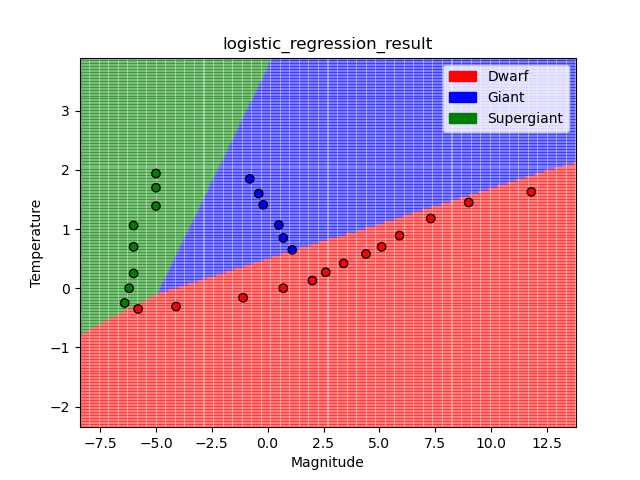
\includegraphics[width=0.475\textwidth]{logistic_regression_result}
			\caption{Logistic Regression Classifier ($\eta = 0.001, \lambda = 0.001$)}
			\label{fig:logistic_regression_classifier}
		\end{figure}
		
		\begin{figure}[h]
			\centering
			\begin{subfigure}[b]{0.475\textwidth}
				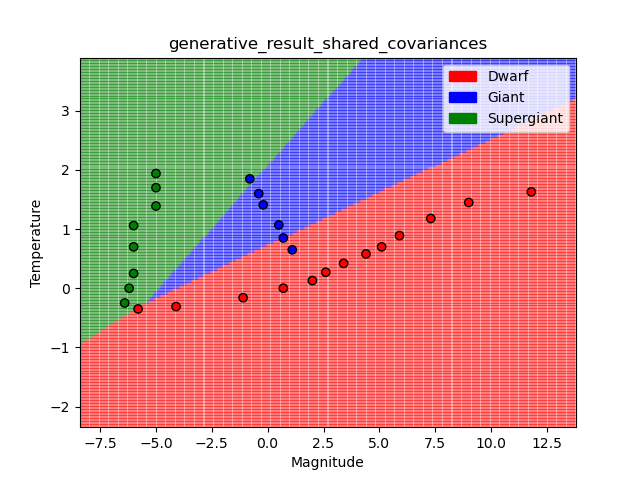
\includegraphics[width=\textwidth]{generative_result_shared_covariances}
			\end{subfigure}
			\hfill
			\begin{subfigure}[b]{0.475\textwidth}
				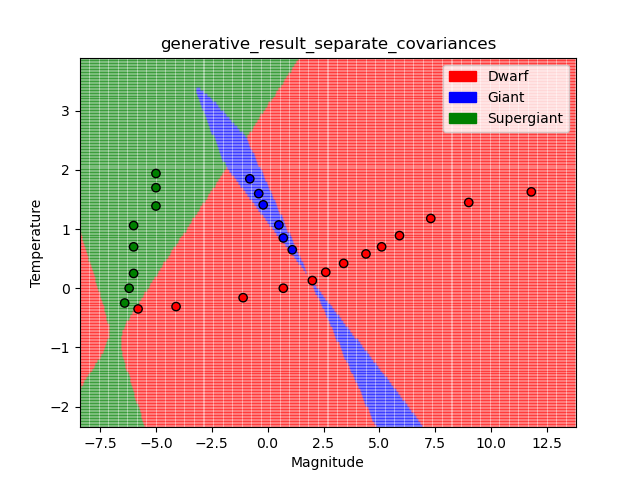
\includegraphics[width=\textwidth]{generative_result_separate_covariances}
			\end{subfigure}
			\caption{Generative Gaussian Classifiers}
			\label{fig:gaussian_classifiers}
		\end{figure}
		
		\begin{figure}[h]
			\centering
			\begin{subfigure}[b]{0.475\textwidth}
				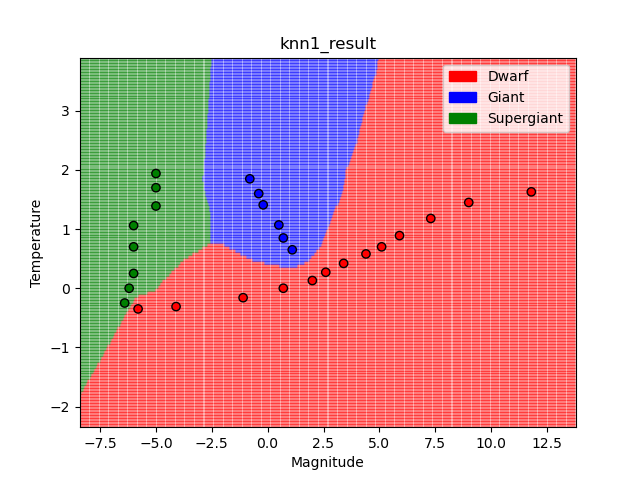
\includegraphics[width=\textwidth]{knn1_result}
			\end{subfigure}
			\hfill
			\begin{subfigure}[b]{0.475\textwidth}
				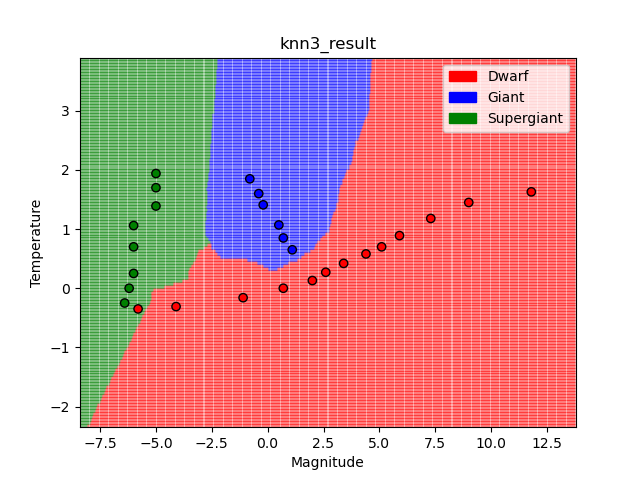
\includegraphics[width=\textwidth]{knn3_result}
			\end{subfigure}
			\hfill
			\vskip\baselineskip
			\begin{subfigure}[b]{0.475\textwidth}
				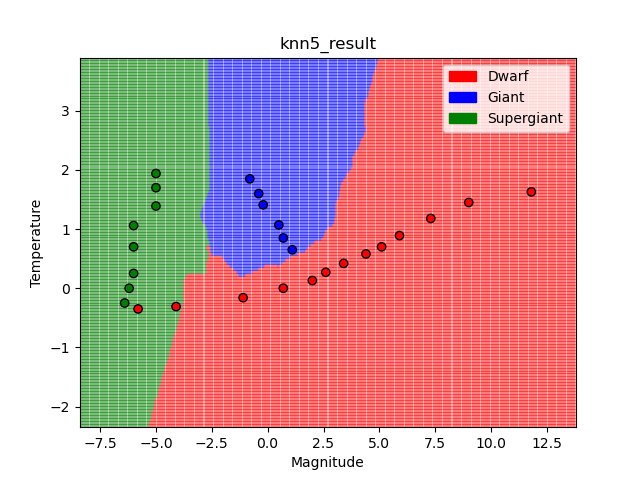
\includegraphics[width=\textwidth]{knn5_result}
			\end{subfigure}
			\caption{KNN Classifiers}
			\label{fig:knn_classifiers}
		\end{figure}

		All of the classifiers do at a good job of fitting the red ``dwarf" and green ``supergiant" points in the training data, but the classifiers vary greatly in the quality of the predictions for the blue ``giant" points. Additionally, the shape and position of the classifiers' decision boundaries vary greatly. The logistic regression and generative Gaussian with shared covariance decision boundaries are very linear and positively correlated and therefore appear to do a relatively poor job of predicting the blue region with its downward trend. This happens because even though these models do have different parameters for the different classes, they are also influenced by information about all of the points overall, because of the gradient calculations and shared covariance matrices. This means that the overall trends of the decision boundaries follow the trends of the majority of points, namely the red and green points. Both of these classifiers have linear boundaries because there are lines where the probability of being in a particular class on either side of the line is even, with the probability increasing for one side or the other when moving away from that line.
		
		The generative model with separate covariances also has somewhat linear decision boundaries, but has much tighter and better prediction regions for the blue and green points, which are roughly symmetric about the line of red points. This is arguably the best classifier since it closely follows the trends of all of the sets of red, blue, and green points separately. The generative model with separate covariances creates these decision boundaries because the shared covariance matrices allow the model to reflect the distinctive variances and covariances within classes that predict, for instance, the negative correlation for the blue class between magnitude and temperature and positive correlations for the other classes between the same two variables. The blue and green regions are symmetric about the plot of red points because points very close to the red training data where it intersects the blue and green training data are more likely to be red, but points slightly farther away can be safely classified as blue or green.
		
		Finally, the KNN classifiers are quite different from the other classifiers because their decision boundaries are all non-linear and curve around the groups of data points for each class. This is because the KNN classifiers make predictions for a given point based on the distance from training points, which results in very curvy prediction boundaries that weave between the classes of points. Because of these curvy prediction lines, the KNN models are able to better reflect the trends of the blue and green points than the logistic regression and generative model with shared covariance. The KNN models are fairly similar for all of the values of $k$ tested, with the main difference being the predictions of the model for the lower left corner of the graph where the green and red training points meet. As $k$ increases, the predictions favor the green points because there are more of these points gathered in that region of the graph. Determining which value of $k$ is best here involves trade-off between the green and red predictions, which is made difficult because the lines of training points appear to intersect. To evenly divide the green and red regions, $k=1$ or $k=3$ seem best.
	
	\item See Figure \ref{fig:logistic_regression_loss}.
		\begin{figure}[h]
			\centering
			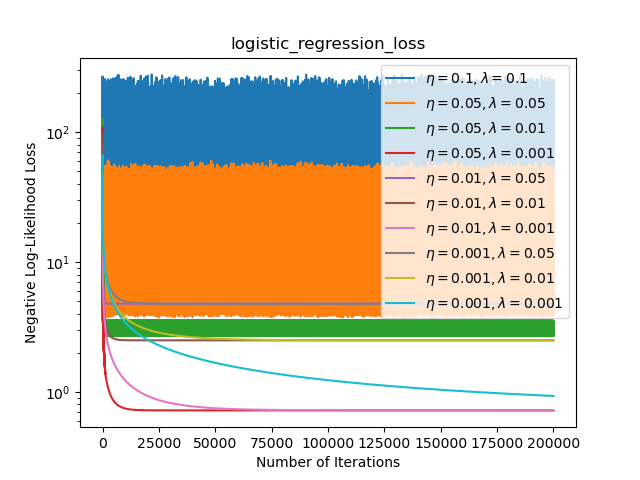
\includegraphics[width=0.7\textwidth]{logistic_regression_loss}
			\caption{Logistic Regression Loss}
			\label{fig:logistic_regression_loss}
		\end{figure}
	
	Based on this plot and looking at the decision boundaries produced by different configurations of hyperparameters, my final choices are $\eta = 0.01$ and $\lambda=0.01$. From the graph, we can see that $\eta=0.1, \lambda=0.1$, $\eta=0.05,\lambda=0.05$, and $\eta=0.05, \lambda=0.01$ do not converge within 200,000 iterations because their learning rate and regularization strength are so high that the loss continually oscillates, making these very bad choices of hyperparameters. The models with the remaining hyperparameters do appear to converge. All three of the models with $\lambda = 0.001$ converge to a loss of zero, however the model with $\eta=0.05$ does so much more quickly than the other models, making it the best choice of the three. The remaining two models with $\lambda=0.05$ converge to a loss of around 4, with the model with $\eta =0.01$ converging faster. Similarly, the remaining two models with $\lambda=0.01$ converge to a loss of around 2.5, with the model with $\eta =0.01$ converging faster. At this point, the best learning rate appears to be $\eta = 0.01$, because it allows fast convergence, while the best regularization strength depends on how much loss we wish to have. This is a potentially difficult choice because minimizing training loss it not necessarily the best choice due to the danger of overfitting. Ultimately I chose $\eta = 0.01, \lambda = 0.01$ as a good middle ground in terms of loss because $\lambda = 0.001$ appeared to slightly overfit the data and $\lambda = 0.05$ appeared to slightly underfit the data.
	
	\item 
	\texttt{Separate Covariance negative log-likelihood: 63.97035984092418 \\
	Shared Covariance negative log-likelihood: 116.39446507788162}
	
	The separate covariance model has a lower loss because having separate covariance information about each class allows the model to be more certain about points that appear to match that class. By contrast, with a shared covariance matrix, these nuances are lost and training class predictions become less certain, and some become incorrect. In particular, the separate covariances matrices allow the model to reflect the positive correlation between features for the red and green points and the negative correlation between the features for the blue points, which are not reflected by the shared covariance matrix. This is evident in the decision boundary plots in Figure \ref{fig:gaussian_classifiers}. With separate covariance matrices, the blue and green regions are grouped much more tightly around the blue and green training points, whereas with shared a shared covariance matrix, the decision boundaries are much looser and the prediction trends are overly general. This leads to higher loss in the shared covariance model, because it does not reflect the training data as well.
	
	\item Consider a star with Magnitude 6 and Temperature 2.
	To what class does each classifier assign this star? Do the
	classifiers give any indication as to whether or not you should
	trust them?
	
	\texttt{Test star type predictions for Separate Covariance Gaussian Model: \\
		magnitude 6 and temperature 2: 0 \\
		Test star type predictions for Shared Covariance Gaussian Model: \\
		magnitude 6 and temperature 2: 1 \\
		Test star type predictions for Linear Regression: \\
		magnitude 6 and temperature 2: 1 \\
		Test star type predictions for KNN Model with k=1: \\
		magnitude 6 and temperature 2: 0 \\
		Test star type predictions for KNN Model with k=3: \\
		magnitude 6 and temperature 2: 0 \\
		Test star type predictions for KNN Model with k=5: \\
		magnitude 6 and temperature 2: 0
	}

	I trust the predictions from the separate covariance Gaussian and KNN models more than those from the shared covariance Gaussian and logistic regression models because the former set of models fit the trainining data better than the latter set, for reasons already described above. In particular, although we don't know the class of this new data point, visually it seems more likely to an outlier dwarf with a high temperature than a giant, because the giants trend downwards and are quite tightly packed together, while the dwarves trend upwards and are closer to this new data point. If we wanted to, we could print out the probabilities for each class returned by the Gaussian and logistic regression models to see how certain each of these classifiers are in their choice for the new data point. If they predicted one class with high probability, we might be more inclined to trust them than if their probabilities were nearly tied between some classes. Somewhat analagously, we could print out the classes of nearest neighbors found by KNN, and see whether there was a clear majority or just a plurality. However, these metrics still reflect the inbuilt biases in the models, so they wouldn't tell us conclusively which predictions to trust.
	
\end{enumerate}

\newpage
%%%%%%%%%%%%%%%%%%%%%%%%%%%%%%%%%%%%%%%%%%%%%
% Name and Calibration
%%%%%%%%%%%%%%%%%%%%%%%%%%%%%%%%%%%%%%%%%%%%%
\subsection*{Name}

Alex Encalada-Stuart

\subsection*{Collaborators and Resources}
Whom did you work with, and did you use any resources beyond cs181-textbook and your notes?

No one and no.

\subsection*{Calibration}
Approximately how long did this homework take you to complete (in hours)?

14

\end{document}
